
\chapter{Methodology}

To achieve the goal of detecting sugar beet plants, the presented YOLOv5 is used. The exact goal is to develop a preprocessing algorithm which standardizes images of sugar beets for a damage prediction regression task. As described, the images should be standardized in a way that each picture contains one sugar beet plant photographed in a $ 90° $ angle to the ground from above. To train the network on the dataset described in the following, a nvidia gpu with 24267 MiB memory was used.

In the following, the given dataset, the training of the network and the evaluation of results will be presented.

\section{Dataset}

There are essentially two sources for images of sugar beets and other plants available. One part consists of images taken in sugar beet fields and the other one is Imagenet \cite{deng2009imagenet} where a large number of different images with classes is available.

The number of images of sugar beet plants is 10087. This set can be categorized in two different types. The first type is an image with many small sugar beets. The other one is an image with older and bigger plants where the concrete object boundaries are hard to see. One example for each class can be seen in figure \ref{fig:image_types}.

\begin{figure}[htb!]
	\centering
	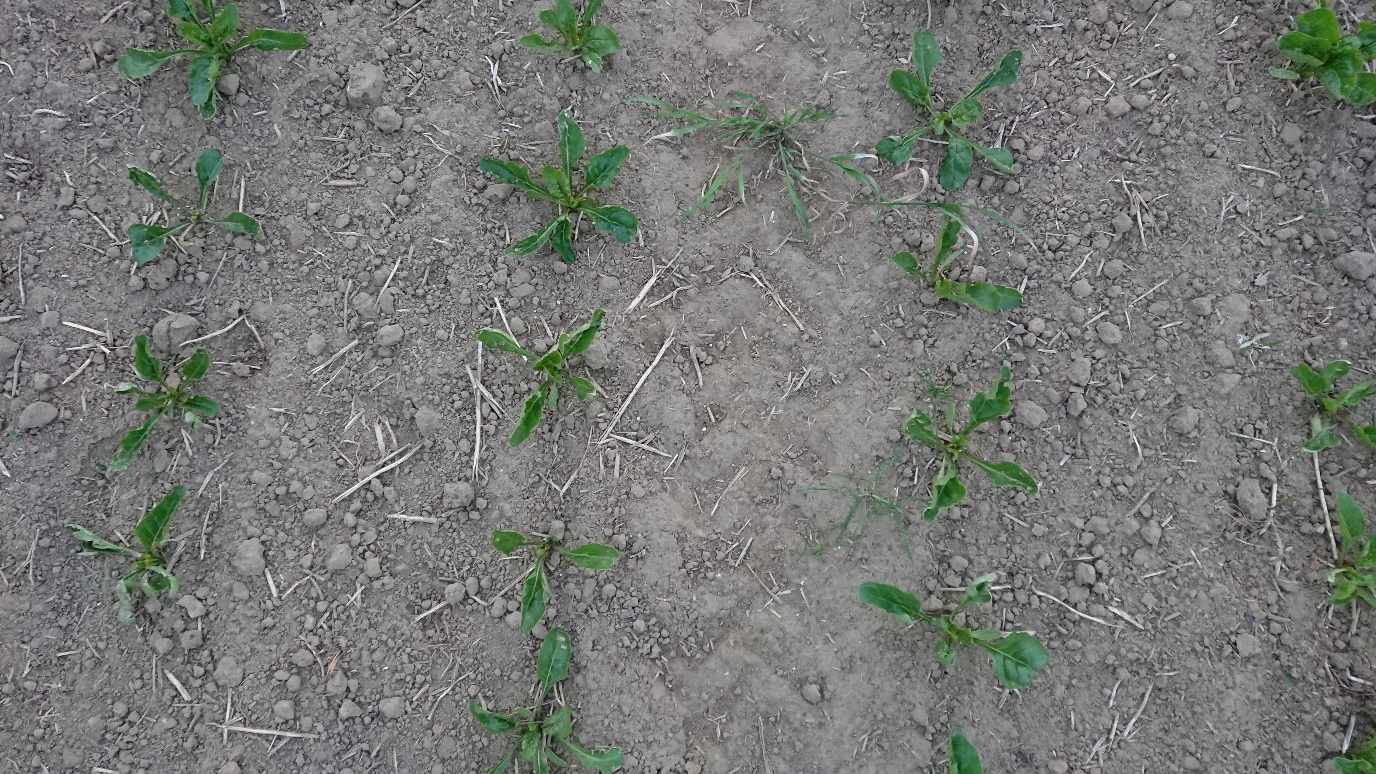
\includegraphics[scale=0.15]{figures/image_type1.JPG}
	\hspace{40pt}
	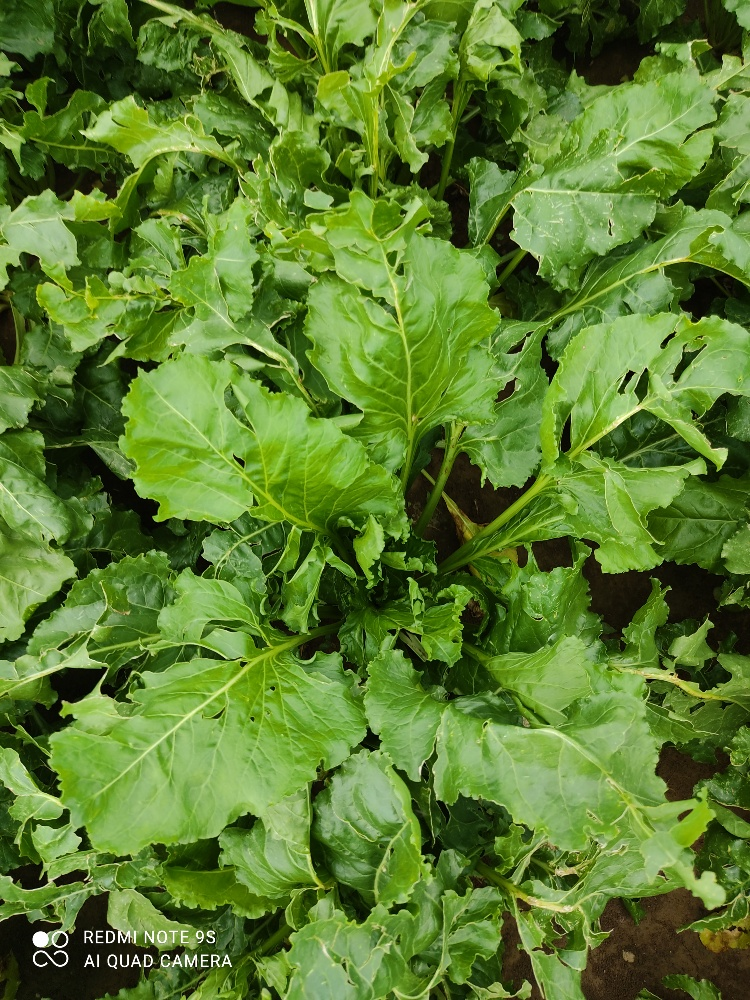
\includegraphics[scale=0.15]{figures/image_type2.jpg}
	\caption{Image types}
	\label{fig:image_types}
\end{figure}

The left one is taken from further away and contains multiple smaller plants. The object boundaries can be seen very clearly. This is not the case for the right example. It contains bigger plants and the boundaries can not be seen clearly because of the neighboring plants. It is not even easy for the human eye to make find the leafs of a distinct plant. The majority of the whole dataset is of the second type (right example). The numbers of images for each type are 9964 for the type of the right example and 123 for the left one. In practice, most images will be of bigger plants because the damage prediction is more important in those cases.\\

To train the network, the pictures have to be labeled. For each image file, one text-file has to be made which contains the information of the image. For each object, one line with five numbers has to be added. The first one is the class. The second and third one are the coordinates of the center of the bounding box (x- and y-coordinate). These have to be relative to the width and height of the image. The third and fourth ones are the length in x- and y-direction. They also have to be relative to the image's height width. First experiments showed that the labeling has to be done manually to obtain reasonable results. It could be seen that only labeling the images with multiple small plants and annotating the other ones automatically with \texttt{0 0.5 0.5 1 1} is not sufficient to detect the exact boundaries of bigger plants. Such a labeling exactly means that the center of the bounding box is in the middle and the boundaries are exactly the same as the image boundaries. In most cases, the whole image was detected as a whole sugar beet plant, which was definitely not the goal. The manual labeling was done with the tool labelImg \cite{labelimg} which provides a graphical user interface to draw the rectangles around the objects. \\

As second source, Imagenet was used. About 3500 images with other plants and flowers were labeled automatically as only one plant other than a sugar beet. Also here, an exact labeling by hands could have been possible but due to time constraints and the fact that only the boundaries of sugar beets have to be detected exactly, this was not done. Further experiments also showed that false positive detections of sugar beets were reduced drastically by including automatically labeled Imagenet pictures. As a third type of images, background images with completely different things on it such as persons, animals or food were also used. Imagenet provides a wide range of data for this use case. These images were just not labeled. 

\section{Training}

\section{Evaluation}
